\documentclass[aspectratio=169,usenames,dvipsnames]{beamer}
\beamertemplatenavigationsymbolsempty
% \documentclass{beamer}

% UNCOMMENT FOR HANDOUTS
% \usepackage{pgfpages}
% \pgfpagesuselayout{2 on 1}[landscape,letterpaper,border shrink=5mm]
% \setbeameroption{show notes}

\mode<presentation>
\usetheme{Boadilla}
\usecolortheme{spruce}
\usepackage{../../LizStyle,ulem}
\usepackage{color}
\usepackage[color,matrix,arrow]{xy}
% \input xy
% \xyoption{all}
\usepackage{tikz}
\usepackage{tikz-cd}
\tikzset{commutative diagrams/diagrams={ampersand replacement=\&}}

\AtBeginSection{\frame{\sectionpage}}


% ==========Command for putting comments and removing them=======
% Visible:
\newcommand{\InstructorNotes}[1]{\textit{\color{orange}#1}}
\newcommand{\InstructorList}[1]{
\begin{itemize}
	\color{orange}
	#1
\end{itemize}
}
% Removed:
% \renewcommand{\InstructorNotes}[1]{}
%\renewcommand{\InstructorList}[1]{}


\newcommand{\bvfill}{\vskip0pt plus 1filll}

\usepackage{multimedia}
\usepackage{graphbox}

% \usepackage{algpseudocode}


\newcommand{\Reeb}{\textbf{Reeb}}
\newcommand{\Rtopc}{\textbf{Rtopc}}
% \newcommand{\RR}{\mathcal{R}}

\newcommand{\Set}{\textbf{Set}}
\newcommand{\Vect}{\textbf{Vect}}
\newcommand{\Top}{\textbf{Top}}
\newcommand{\Int}{\textbf{Int}}


\graphicspath{ {Figures/} {../Figures/}{../../Figures/} }



\begin{document}
%\pdfoptionpdfminorversion 5
%\logo{\includegraphics[height=1.5cm]{dukeshield.pdf}}
\title[]{Ch 5.1.5: $k$-fold Cross-Validation for Classification}
\subtitle{Lecture 15 - CMSE 381}
\date{Fri, Feb 20, 2026}



\institute[MSU-CMSE]{Michigan State University\\
			::\\
          Dept of Computational Mathematics, Science \& Engineering}


\begin{frame}
 \titlepage


\end{frame}
%--------------------------
\begin{frame}[c]{Announcements}

\begin{columns}
\column{.45\textwidth}
\centering

	\textbf{Last time:}
	\begin{itemize}
		\item k-fold CV
	\end{itemize}
	\textbf{This lecture:}
	\begin{itemize}
		\item CV for classification
	\end{itemize}
\column{.45\textwidth}

\centering

\textbf{Announcements:}
	\begin{itemize}
		\item Homework \#3 is due Sunday 3/8
		% \item Grades \\
		% 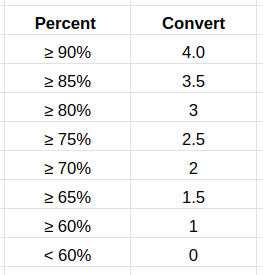
\includegraphics[width = .6\textwidth]{GradeConversion}
	\end{itemize}
\end{columns}

\end{frame}
%--- Next Frame ---%

%=================
\section{Last time}
%=================

\begin{frame}[t]{Approximations of Test Error}
\begin{columns}
\column{.3\textwidth}
\centering
\textbf{Validation Set}
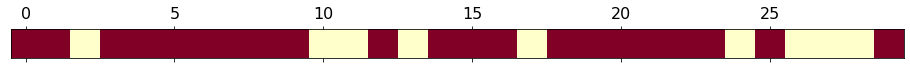
\includegraphics[width = \textwidth]{CV-subset0}
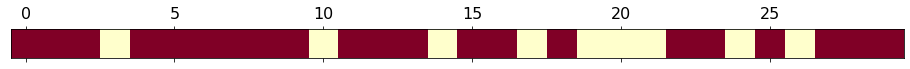
\includegraphics[width = \textwidth]{CV-subset1}
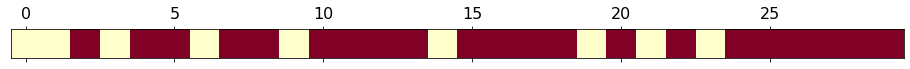
\includegraphics[width = \textwidth]{CV-subset2}
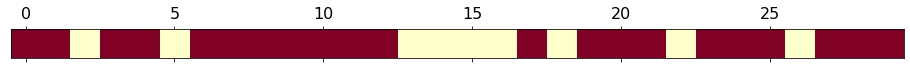
\includegraphics[width = \textwidth]{CV-subset3}
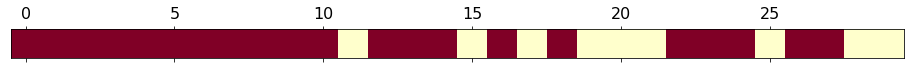
\includegraphics[width = \textwidth]{CV-subset4}
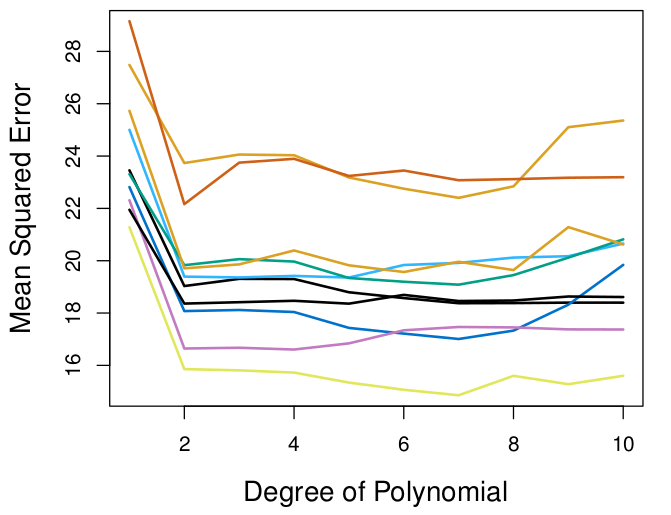
\includegraphics[width = .8\textwidth]{Fig5-2b}
\column{.3\textwidth}
\centering
\textbf{LOOCV}
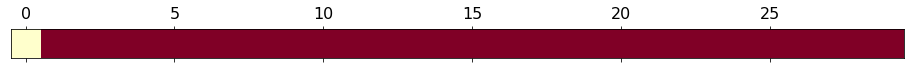
\includegraphics[width = \textwidth]{LOOCV-subset0.png}

\includegraphics[width = \textwidth]{LOOCV-subset1.png}

\includegraphics[width = \textwidth]{LOOCV-subset2.png}
% 
\includegraphics[width = \textwidth]{LOOCV-subset3.png}
% 
\includegraphics[width = \textwidth]{LOOCV-subset4.png}
$\vdots$

\includegraphics[width = \textwidth]{LOOCV-subset29.png}

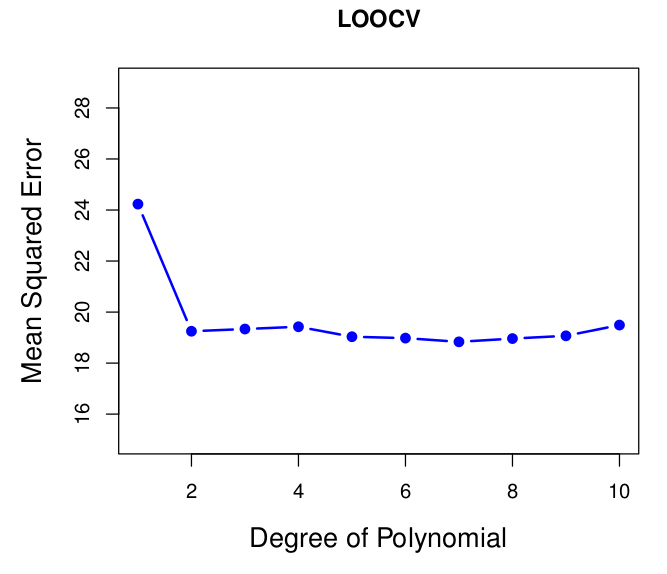
\includegraphics[width = .8\textwidth]{Fig5-4a}

\column{.3\textwidth}
\centering
\textbf{K-fold CV}
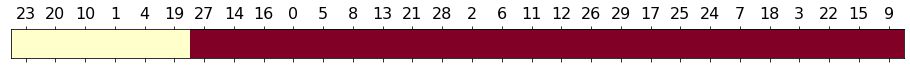
\includegraphics[width = \textwidth]{CV-Kfold-subset0}

\includegraphics[width = \textwidth]{CV-Kfold-subset1}

\includegraphics[width = \textwidth]{CV-Kfold-subset2}

\includegraphics[width = \textwidth]{CV-Kfold-subset3}

\includegraphics[width = \textwidth]{CV-Kfold-subset4}
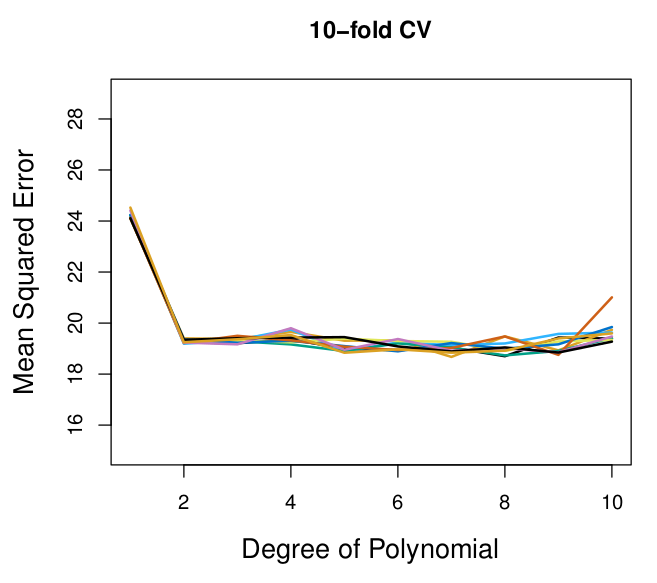
\includegraphics[width = .8\textwidth, align = c]{Fig5-4b}
\end{columns}
\end{frame}
%--- Next Frame ---%



%--- Next Frame ---%
\begin{frame}[c]{Definition of $k$-fold CV}

\begin{columns}
\column{.45\textwidth}
\centering
\begin{itemize}
	\item Randomly split data into $k$-groups (folds)
	\item Approximately equal sized. For the sake of notation, say each set has $\ell$ points
	\item []
	\item Remove $i$th fold $U_i$ and reserve for testing.
	\item Train the model on remaining points
	\item Calculate $\mathrm{MSE}_i = \frac{1}{\ell} \sum_{(x_j,y_j) \in U_i}(y_j-\hat y_j)^2$
	\item[]
	\item Rinse and repeat
\end{itemize}
\column{.45\textwidth}
\centering
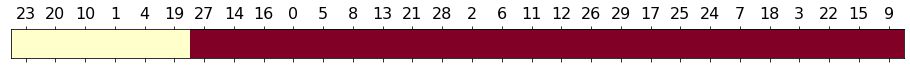
\includegraphics[width = \textwidth]{CV-Kfold-subset0}

\includegraphics[width = \textwidth]{CV-Kfold-subset1}

\includegraphics[width = \textwidth]{CV-Kfold-subset2}

\includegraphics[width = \textwidth]{CV-Kfold-subset3}

\includegraphics[width = \textwidth]{CV-Kfold-subset4}
Return
\begin{equation*}
	CV_{(k)} = \frac{1}{k} \sum_{i=1}^k \mathrm{MSE}_i
\end{equation*}
\end{columns}

\end{frame}
%--- Next Frame ---%


%=====
\section{CV for Classification}
%=====

\begin{frame}[c]{Setup: LOOCV}

	\begin{columns}
	\column{.45\textwidth}
	\centering
	\begin{itemize}
		\item Remove $i$th point $(x_i,y_i)$ and reserve for testing.
		\item Train the model on remaining points
		\item Calculate $\mathrm{Err}_i = \mathrm{I}(y_j\neq\hat y_j)$
		\item[]
		\item Rinse and repeat
	\end{itemize}
	\column{.45\textwidth}
	\centering
	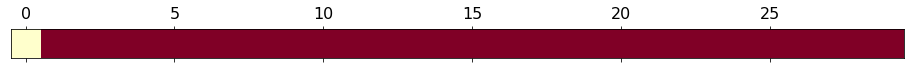
\includegraphics[width = \textwidth]{LOOCV-subset0.png}
	
\includegraphics[width = \textwidth]{LOOCV-subset1.png}
	
\includegraphics[width = \textwidth]{LOOCV-subset2.png}
	
\includegraphics[width = \textwidth]{LOOCV-subset3.png}
	
\includegraphics[width = \textwidth]{LOOCV-subset4.png}
	$\vdots$
	
\includegraphics[width = \textwidth]{LOOCV-subset29.png}
	Return
	\begin{equation*}
		CV_{(n)} = \frac{1}{n} \sum_{i=1}^n \mathrm{Err}_i
	\end{equation*}
	\end{columns}

\end{frame}
%--- Next Frame ---%
\begin{frame}[c]{Setup: $k$-fold}

	\begin{columns}
	\column{.45\textwidth}
	\centering
	\begin{itemize}
		\item Randomly split data into $k$-groups (folds)
		\item Approximately equal sized. For the sake of notation, say each set has $\ell$ points
		\item []
		\item Remove $i$th fold $U_i$ and reserve for testing.
		\item Train the model on remaining points
		\item Calculate $\mathrm{Err}_i = \frac{1}{\ell} \sum_{(x_j,y_j) \in U_i}\mathrm{I}(y_j\neq\hat y_j)$
		\item[]
		\item Rinse and repeat
	\end{itemize}
	\column{.45\textwidth}
	\centering
	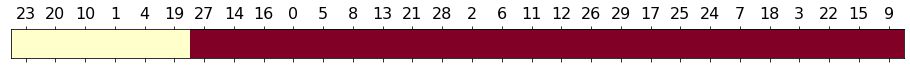
\includegraphics[width = \textwidth]{CV-Kfold-subset0}
	
\includegraphics[width = \textwidth]{CV-Kfold-subset1}
	
\includegraphics[width = \textwidth]{CV-Kfold-subset2}
	
\includegraphics[width = \textwidth]{CV-Kfold-subset3}
	
\includegraphics[width = \textwidth]{CV-Kfold-subset4}

	Return
	\begin{equation*}
		CV_{(k)} = \frac{1}{k} \sum_{i=1}^k \mathrm{Err}_i
	\end{equation*}
	\end{columns}

\end{frame}
%--- Next Frame ---%
\begin{frame}[c]{Example on simulated data: Linear}

\begin{columns}
\column{.4\textwidth}
\centering
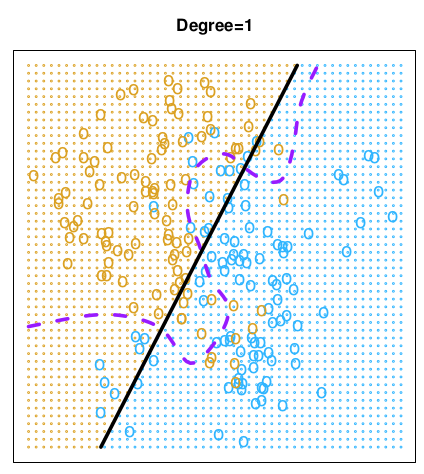
\includegraphics[width = \textwidth]{Fig5-7a}
\column{.45\textwidth}
\centering
\begin{itemize}
	\item Purple: Bayes decision boundary.
	\begin{itemize}
		\item Error rate: 0.133
	\end{itemize}
	\item Black: Logistic regression
	\begin{itemize}
	\item $\log(p/(1-p)) = \beta_0 + \beta_1X_1 + \beta_2 X_2$
	\item Error rate: 0.201
	\end{itemize}
\end{itemize}
\InstructorList{
\item remind them the boundary is essential $p=(1-p)$, meaning $\beta_0 + \beta_1X_1 + \beta_2 X_2=0$
\item No k-fold yet
\item Error rate for logistic still high, so not great job yet
\item So, up the degree and see what happens
}
\end{columns}

\end{frame}
%--- Next Frame ---%
\begin{frame}[c]{Example on simulated data: Quadratic logistic regression}

\begin{columns}
\column{.4\textwidth}
\centering
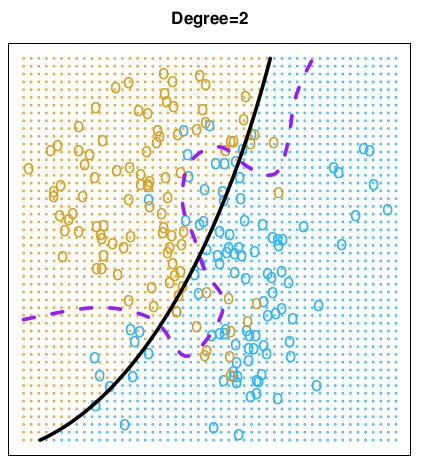
\includegraphics[width = \textwidth]{Fig5-7b}
\column{.45\textwidth}
\centering
\begin{itemize}
	\item Purple: Bayes decision boundary.
	\begin{itemize}
		\item Error rate: 0.133
	\end{itemize}
	\item Black: Logistic regression
	\begin{itemize}
	\item $\log(p/(1-p)) = \beta_0 + \beta_1X_1 + \beta_2X_1^2 + \beta_3 X_2 + \beta_4X_2^2$
	\item Error rate: 0.197
	\end{itemize}
\end{itemize}
\InstructorList{
\item No k-fold yet
\item Error rate for logistic slight improvement, but still not great
\item So, up the degree again and see what happens
}
\end{columns}

\end{frame}
%--- Next Frame ---%
\begin{frame}[c]{Example on simulated data: all the polynomials!}

\begin{columns}
\column{.45\textwidth}
\centering
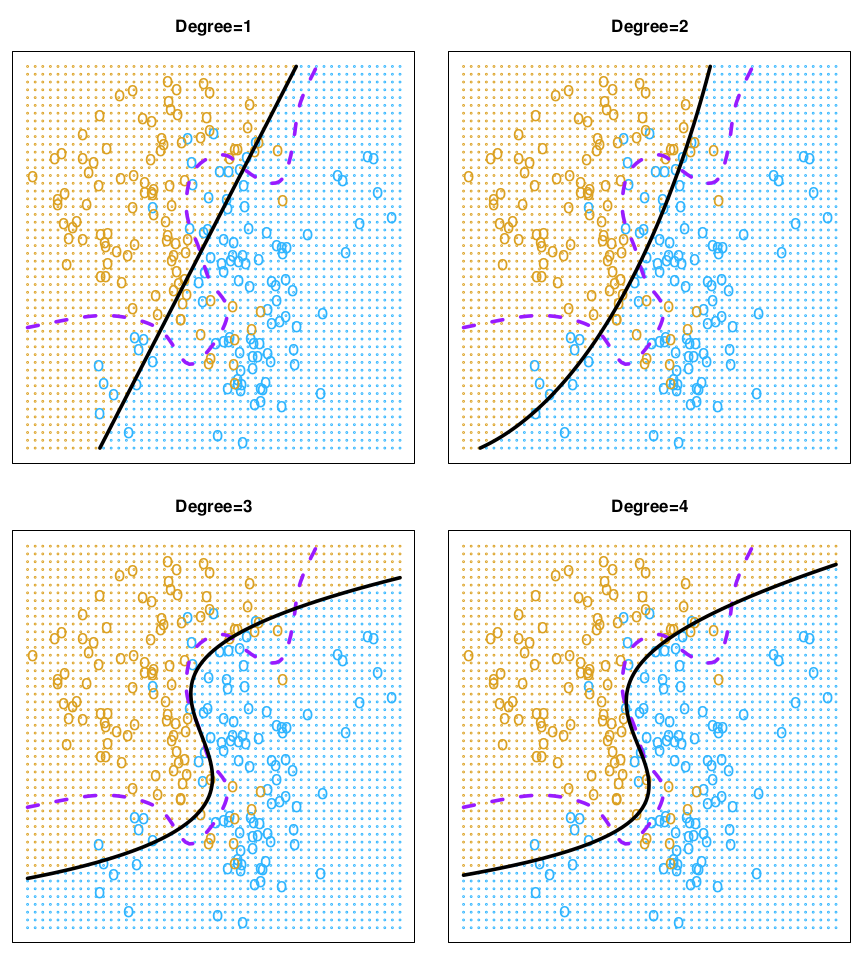
\includegraphics[width = \textwidth]{Fig5-7}
\column{.35\textwidth}
\centering
\begin{itemize}
	\item Purple: Bayes decision boundary.
	\begin{itemize}
		\item Error rate: 0.133
	\end{itemize}
	\item Black: Logistic regression
	\begin{itemize}
	\item Deg 1 Error rate: 0.201
	\item Deg 2 Error rate: 0.197
	\item Deg 3 Error rate: 0.160
	\item Deg 4 Error rate: 0.162
	\end{itemize}
	\end{itemize}
	\InstructorList{
	\item Normally, we don't have the Bayes decision boundary
	\item How do you pick between models?
	}
\end{columns}

\end{frame}
%--- Next Frame ---%
\begin{frame}[c]{Decide degree based on CV}

\begin{columns}
\column{.45\textwidth}
\centering
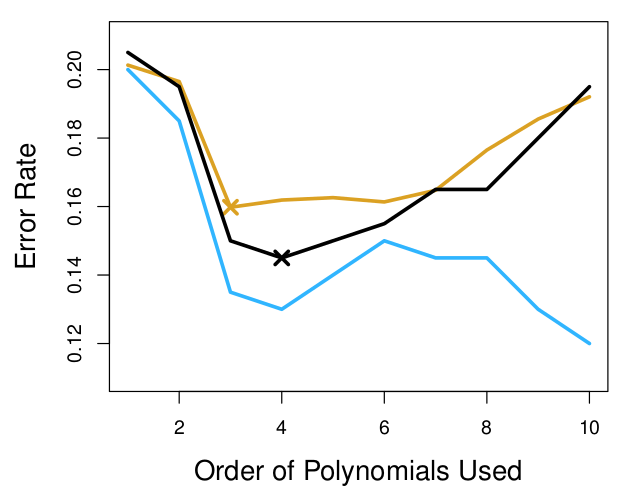
\includegraphics[width = \textwidth]{Fig5-8a}
\column{.5\textwidth}
\centering
\begin{itemize}
	\item Test error (brown)
	\item Training error (blue)
	\item 10-fold CV error (black)
\end{itemize}
\footnotesize
\InstructorList{
\item Training error tends to decrease as the flexibility of the fit increases.
\item Note decrease in blue isn't monotonic, but still going down overall
\item test error displays a characteristic U-shape.
\item The 10-fold CV provides a pretty good (but underestimate) approximation to the test error rate.
\item minimum at 4, close to minimum of test curve at 3
}
\end{columns}

\end{frame}
%--- Next Frame ---%
\begin{frame}[c]{Similar game for KNN}

\begin{columns}
\column{.45\textwidth}
\centering
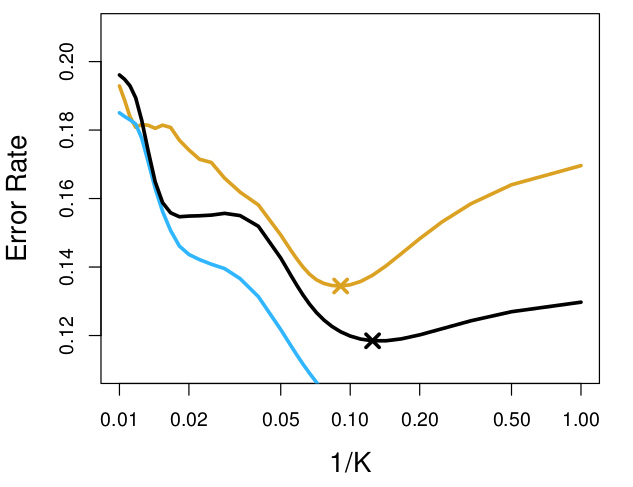
\includegraphics[width = \textwidth]{Fig5-8b}
\column{.45\textwidth}
\centering
\begin{itemize}
	\item Test error (brown)
	\item Training error (blue)
	\item 10-fold CV error (black)
\end{itemize}
\InstructorList{
\item Note that using a different changing parameter
\item similar idea to figure out the right choice of $K$.
\item Minimm in black (10 fold CV) has $1/K$ value close to where brown does, so good choice
}
\end{columns}

\end{frame}
%--- Next Frame ---%
{
\setbeamercolor{background canvas}{bg=Apricot!25}
\begin{frame}[t]{Coding - k-fold for penguin classification section }
\begin{columns}
\column{.45\textwidth}
\centering
\column{.45\textwidth}
\centering
\end{columns}
\end{frame}
}
%--- Next Frame ---%
\begin{frame}[c]{TL;DR}

\begin{columns}
\column{.45\textwidth}
\centering
$k$-fold CV
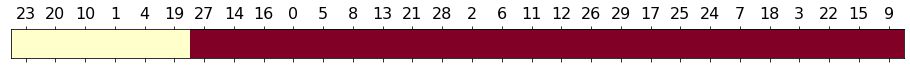
\includegraphics[width = \textwidth]{CV-Kfold-subset0}

\includegraphics[width = \textwidth]{CV-Kfold-subset1}

\includegraphics[width = \textwidth]{CV-Kfold-subset2}

\includegraphics[width = \textwidth]{CV-Kfold-subset3}

\includegraphics[width = \textwidth]{CV-Kfold-subset4}
\begin{equation*}
	CV_{(k)} = \frac{1}{k} \sum_{i=1}^k \mathrm{MSE}_i
\end{equation*}

Use $k=5$ or 10 usually
\column{.45\textwidth}
\centering
$k$-fold CV for classification
\begin{equation*}
\mathrm{Err}_i = \mathrm{I}(y_j\neq\hat y_j)
\end{equation*}
\begin{equation*}
	CV_{(k)} = \frac{1}{k} \sum_{i=1}^k \mathrm{Err}_i
\end{equation*}


\end{columns}

\end{frame}
%--- Next Frame ---%
% %----------------
\begin{frame}[t]{Next time}


	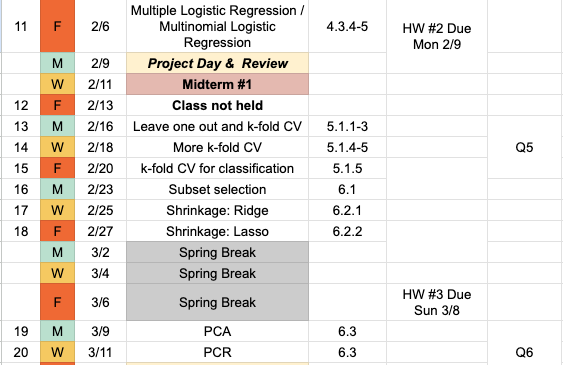
\includegraphics[align = c, width = .65\textwidth]{Schedule-S26-Lecs11_to_20}
\begin{columns}
\column{.45\textwidth}
\centering


\column{.45\textwidth}

\end{columns}
\end{frame}
%--- Next Frame ---%


\end{document}
